%!TEX root = ../dissertation.tex

\chapter{Methodology}
\label{chp:methodology}
This chapter outlines the methodology employed in the development and implementation of the Social Media Kit (SMKIT) project. It provides a comprehensive explanation of the tools, techniques, and processes used to design, build, and implement the system. The chapter begins with an overview of the system architecture, followed by detailed discussions on data collection, processing, and the integration of various components.
This chapter sets the foundation for understanding the practical implementation of SMKIT, which will be further detailed in the subsequent chapters.


\section{Introduction}
\label{sec:methodology_introduction}
This section introduces the methodology used for developing the Social Media Kit (SMKIT). It provides an overview of the key techniques and tools employed throughout the development process, providing the foundation for the work presented in this thesis. The methodology chapter serves as a detailed explanation of how the objectives of SMKIT were achieved, with a focus on the following key areas:

\begin{itemize}
    \item \textbf{System Design and Architecture}: A comprehensive description of the system architecture of SMKIT, including the design decisions made to ensure the system’s scalability and functionality.
    \item \textbf{Data Collection and Preparation}: An overview of the data extraction techniques used, including web scraping tools and methods for cleaning and transforming the data into usable formats.
    \item \textbf{Implementation Process}: A detailed explanation of the implementation phase, where the system was developed and integrated with components like Negapedia and social media platforms.
    \item \textbf{Challenges and Limitations}: A reflection on the obstacles faced during the project and the limitations of the system that are important to consider when interpreting the results.
\end{itemize}

Each of these areas will be explored in detail in the subsequent sections of this chapter. By providing a comprehensive explanation of the methodologies used, this chapter ensures that the development process of SMKIT is well-understood.

The following sections will build upon this introductory overview, examining each of the mentioned aspects in greater detail to provide a complete picture of the technical and conceptual approaches adopted in the development of SMKIT.


\section{System Design and Architecture}
\label{sec:system_design_and_architecture}
This section explains the design decisions made for the Social Media Kit (SMKIT), including the overall system architecture, the key components that make up the system, and how these components interact to achieve the desired functionality. The system is designed to automate the generation and sharing of content on social media platforms, leveraging data from websites that integrate Open Graph (OG) tags or from the Negapedia website through a dedicated module for contextual analysis and content creation.

The architecture of SMKIT is based on a modular and scalable approach, allowing for flexibility in future development. Below are the key aspects of the system design:

\begin{itemize}
    \item \textbf{Modular Architecture}: The system is built using a modular architecture, where each component or unit has a specific responsibility. This allows for easy maintenance and the potential for future upgrades. \begin{comment} The key components include:
    \begin{itemize}
        \item \textbf{Data Extraction Component}: Responsible for extracting data from external sources, such as websites with Open Graph (OG) tags or Negapedia specific data through web scraping.
        \item \textbf{Data Transformation Component}: Handles data cleaning, transformation, and analysis, converting raw data into structured and usable formats.
        \item \textbf{Content Creation Component}: Uses the processed data to automatically generate content for social media posts, including text and multimedia.
        \item \textbf{Social Media Posting Component}: Manages the process of posting content, previously extracted into structured and usable formats, to various social media platforms (e.g., Twitter, Facebook) through the use of APIs.
    \end{itemize} \end{comment}
    
    
    \item \textbf{Scalability}: SMKIT is designed with scalability in mind. The system can handle multiple social media platforms and expand to include additional sources of data and content generation features. By using a modular structure, new components can be added without disrupting existing functionality.
    
    \item \textbf{Data Flow}: The data flow in SMKIT is sequential and structured. The process begins with the extraction of data from external sources, followed by cleaning and transformation, content generation, and finally, posting to social media platforms. \begin{comment} The following diagram illustrates the flow of data through the system:
    
    \begin{figure}[ht]
        \centering
        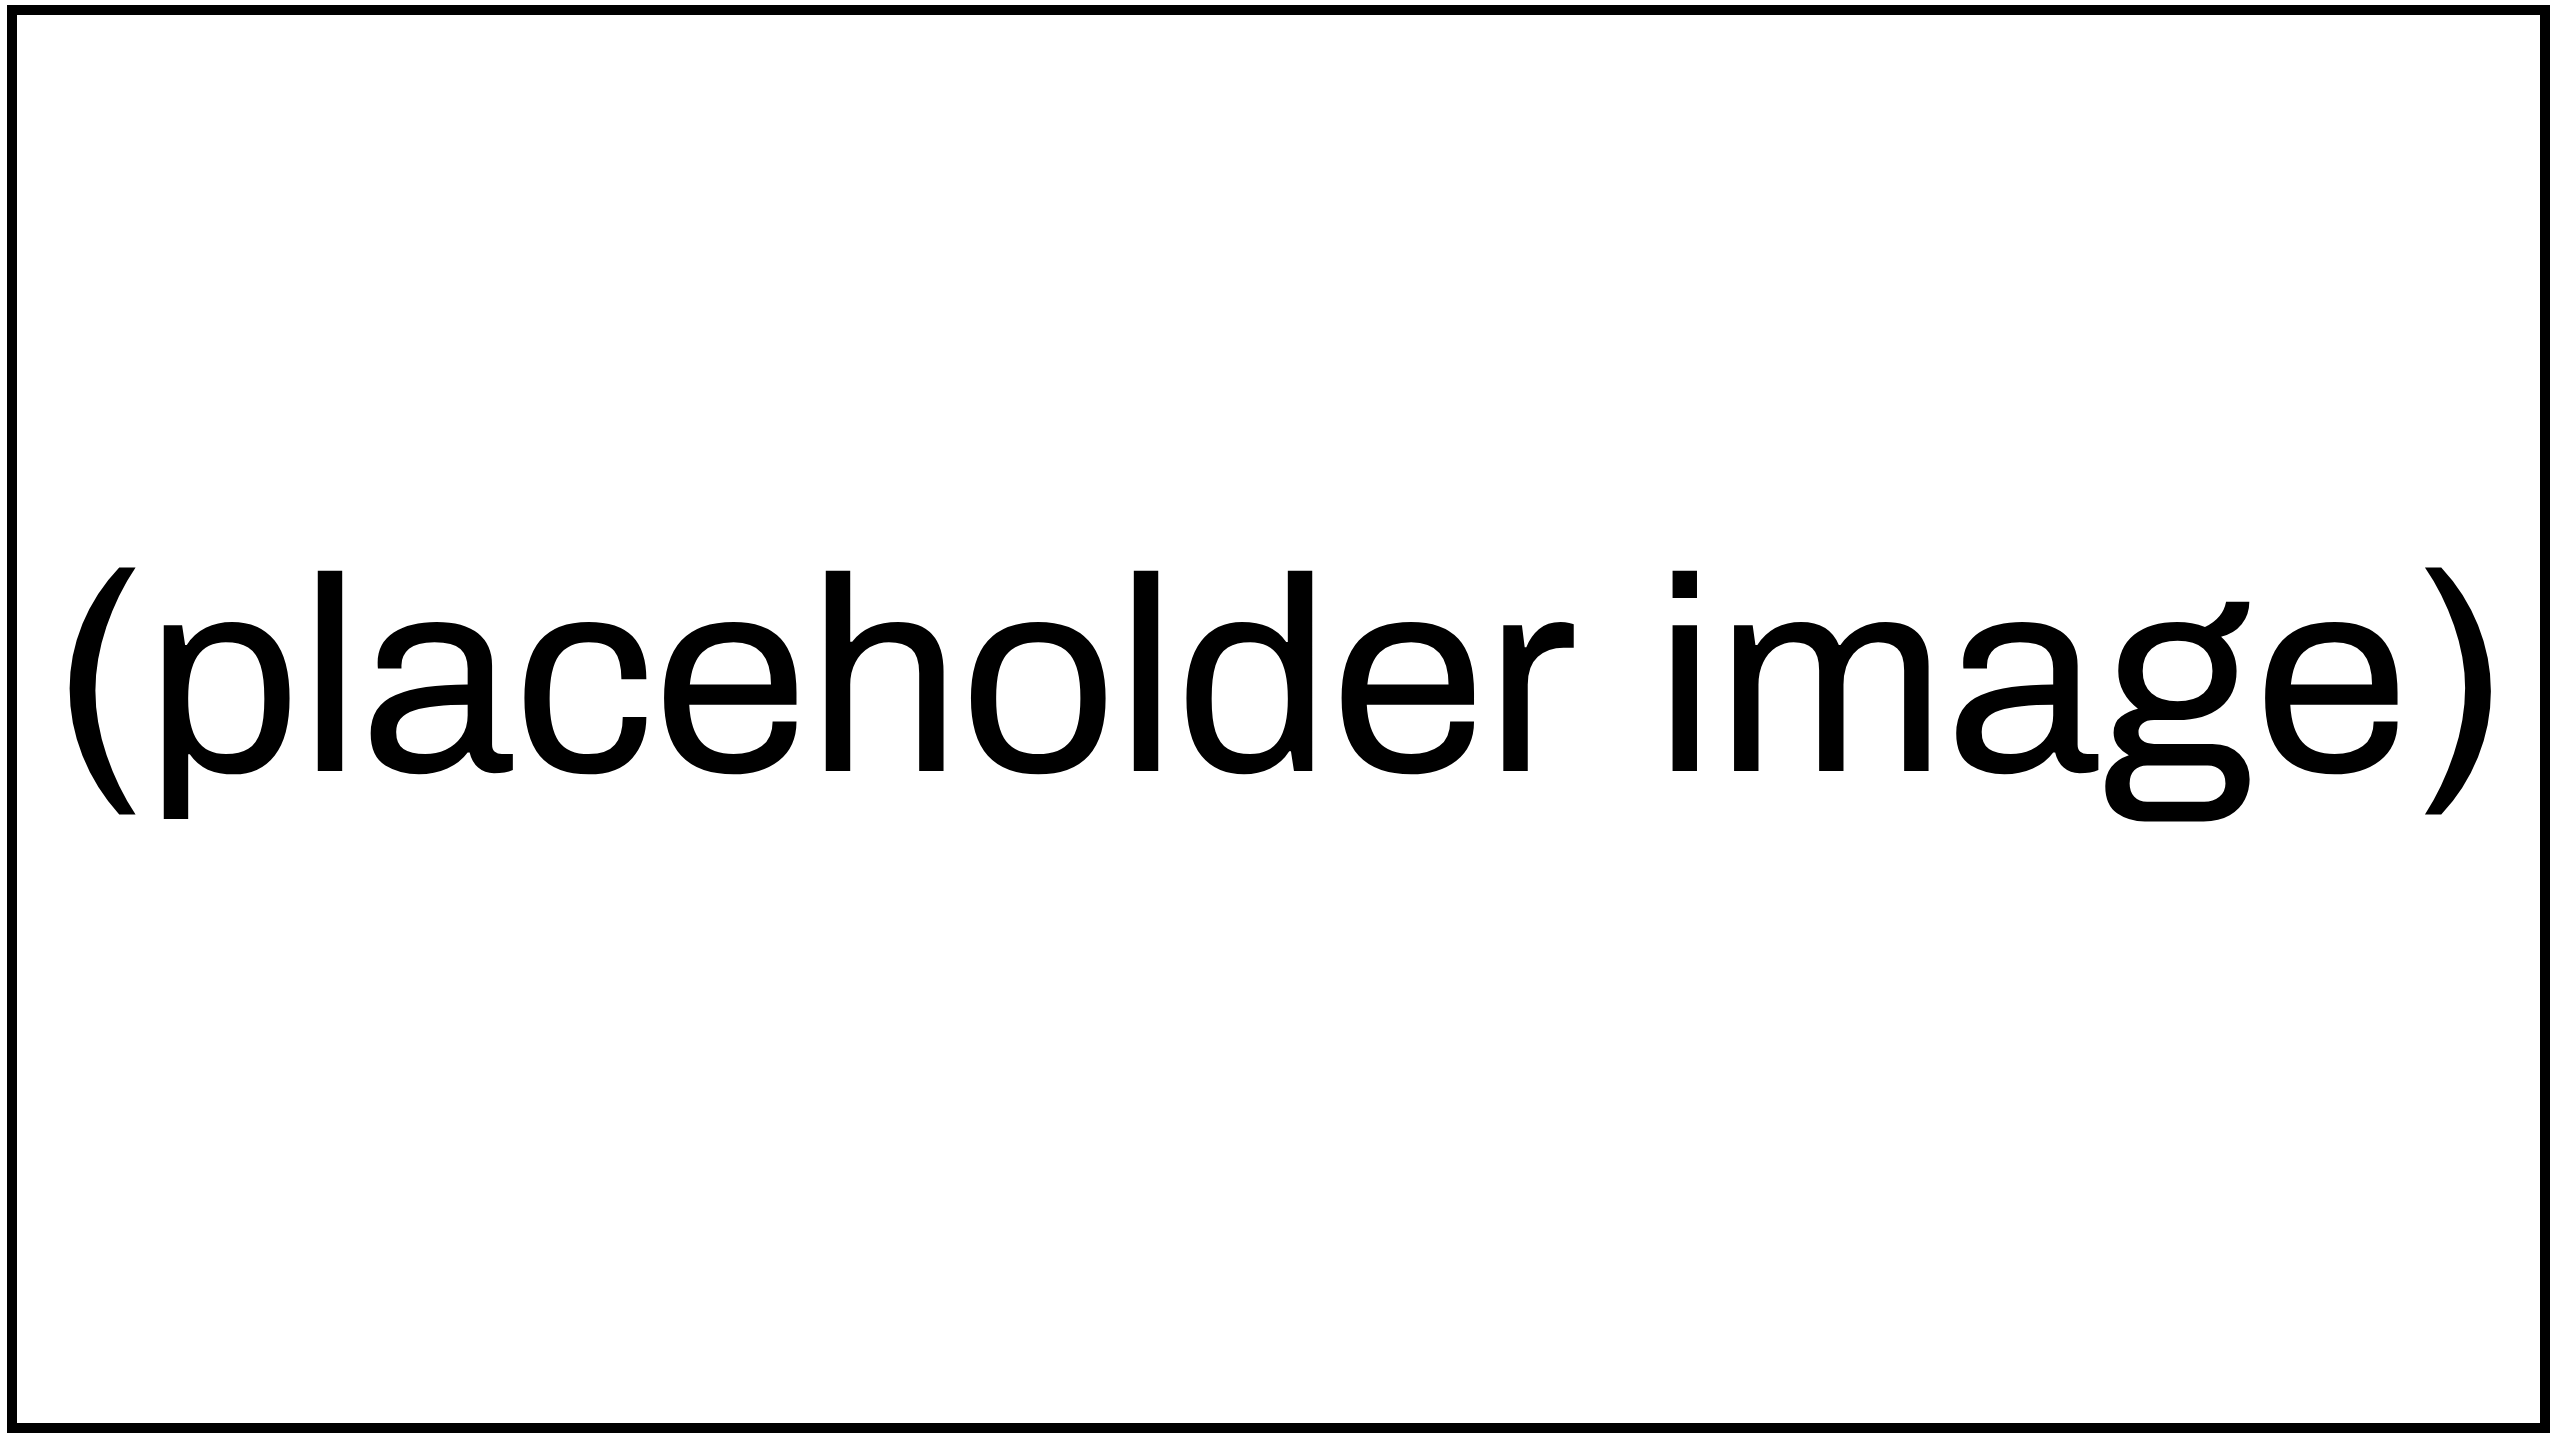
\includegraphics[width=0.8\textwidth]{figures/methodology/placeholder_image.png}
        \caption{System Architecture and Data Flow}
        \label{fig:system_architecture}
    \end{figure} \end{comment}

\end{itemize}

\subsection{System Architecture Overview}
\label{subsec:system_architecture_overview}
The system architecture of the Social Media Kit (SMKIT) is designed with a modular approach to ensure scalability, flexibility, and ease of maintenance. The architecture integrates several key components that work together to automate the extraction, processing, generation, and sharing of content on social media platforms. Below is an overview of how these components interact:

\begin{itemize}
    \item \textbf{Data Extraction Component}: The system begins by extracting raw data from external sources. This data extraction process can be achieved through web scraping, which provide the foundational content for further processing.

    \item \textbf{Data Transformation Component}: Once the raw data is collected, it is passed on to the data transformation component. This component is responsible for cleaning, structuring, and transforming the raw data into a usable format. It processes unstructured text to extract key insights, removes irrelevant or noisy data, and organizes the content into predefined formats.
    
    \item \textbf{Social Media Posting Component}: Finally, the transformed content is sent to the social media posting component. This component manages the process of sharing the content across various platforms like Twitter and Facebook, utilizing platform-specific APIs to ensure seamless posting.
\end{itemize}

The modularity of the architecture allows for flexibility in extending the system to include new data sources with eventually new tailored predefined formats, additional social media platforms, or advanced content generation techniques, such as sentiment analysis and machine learning-based content optimization.

\begin{comment}
\begin{figure}[ht]
    \centering
    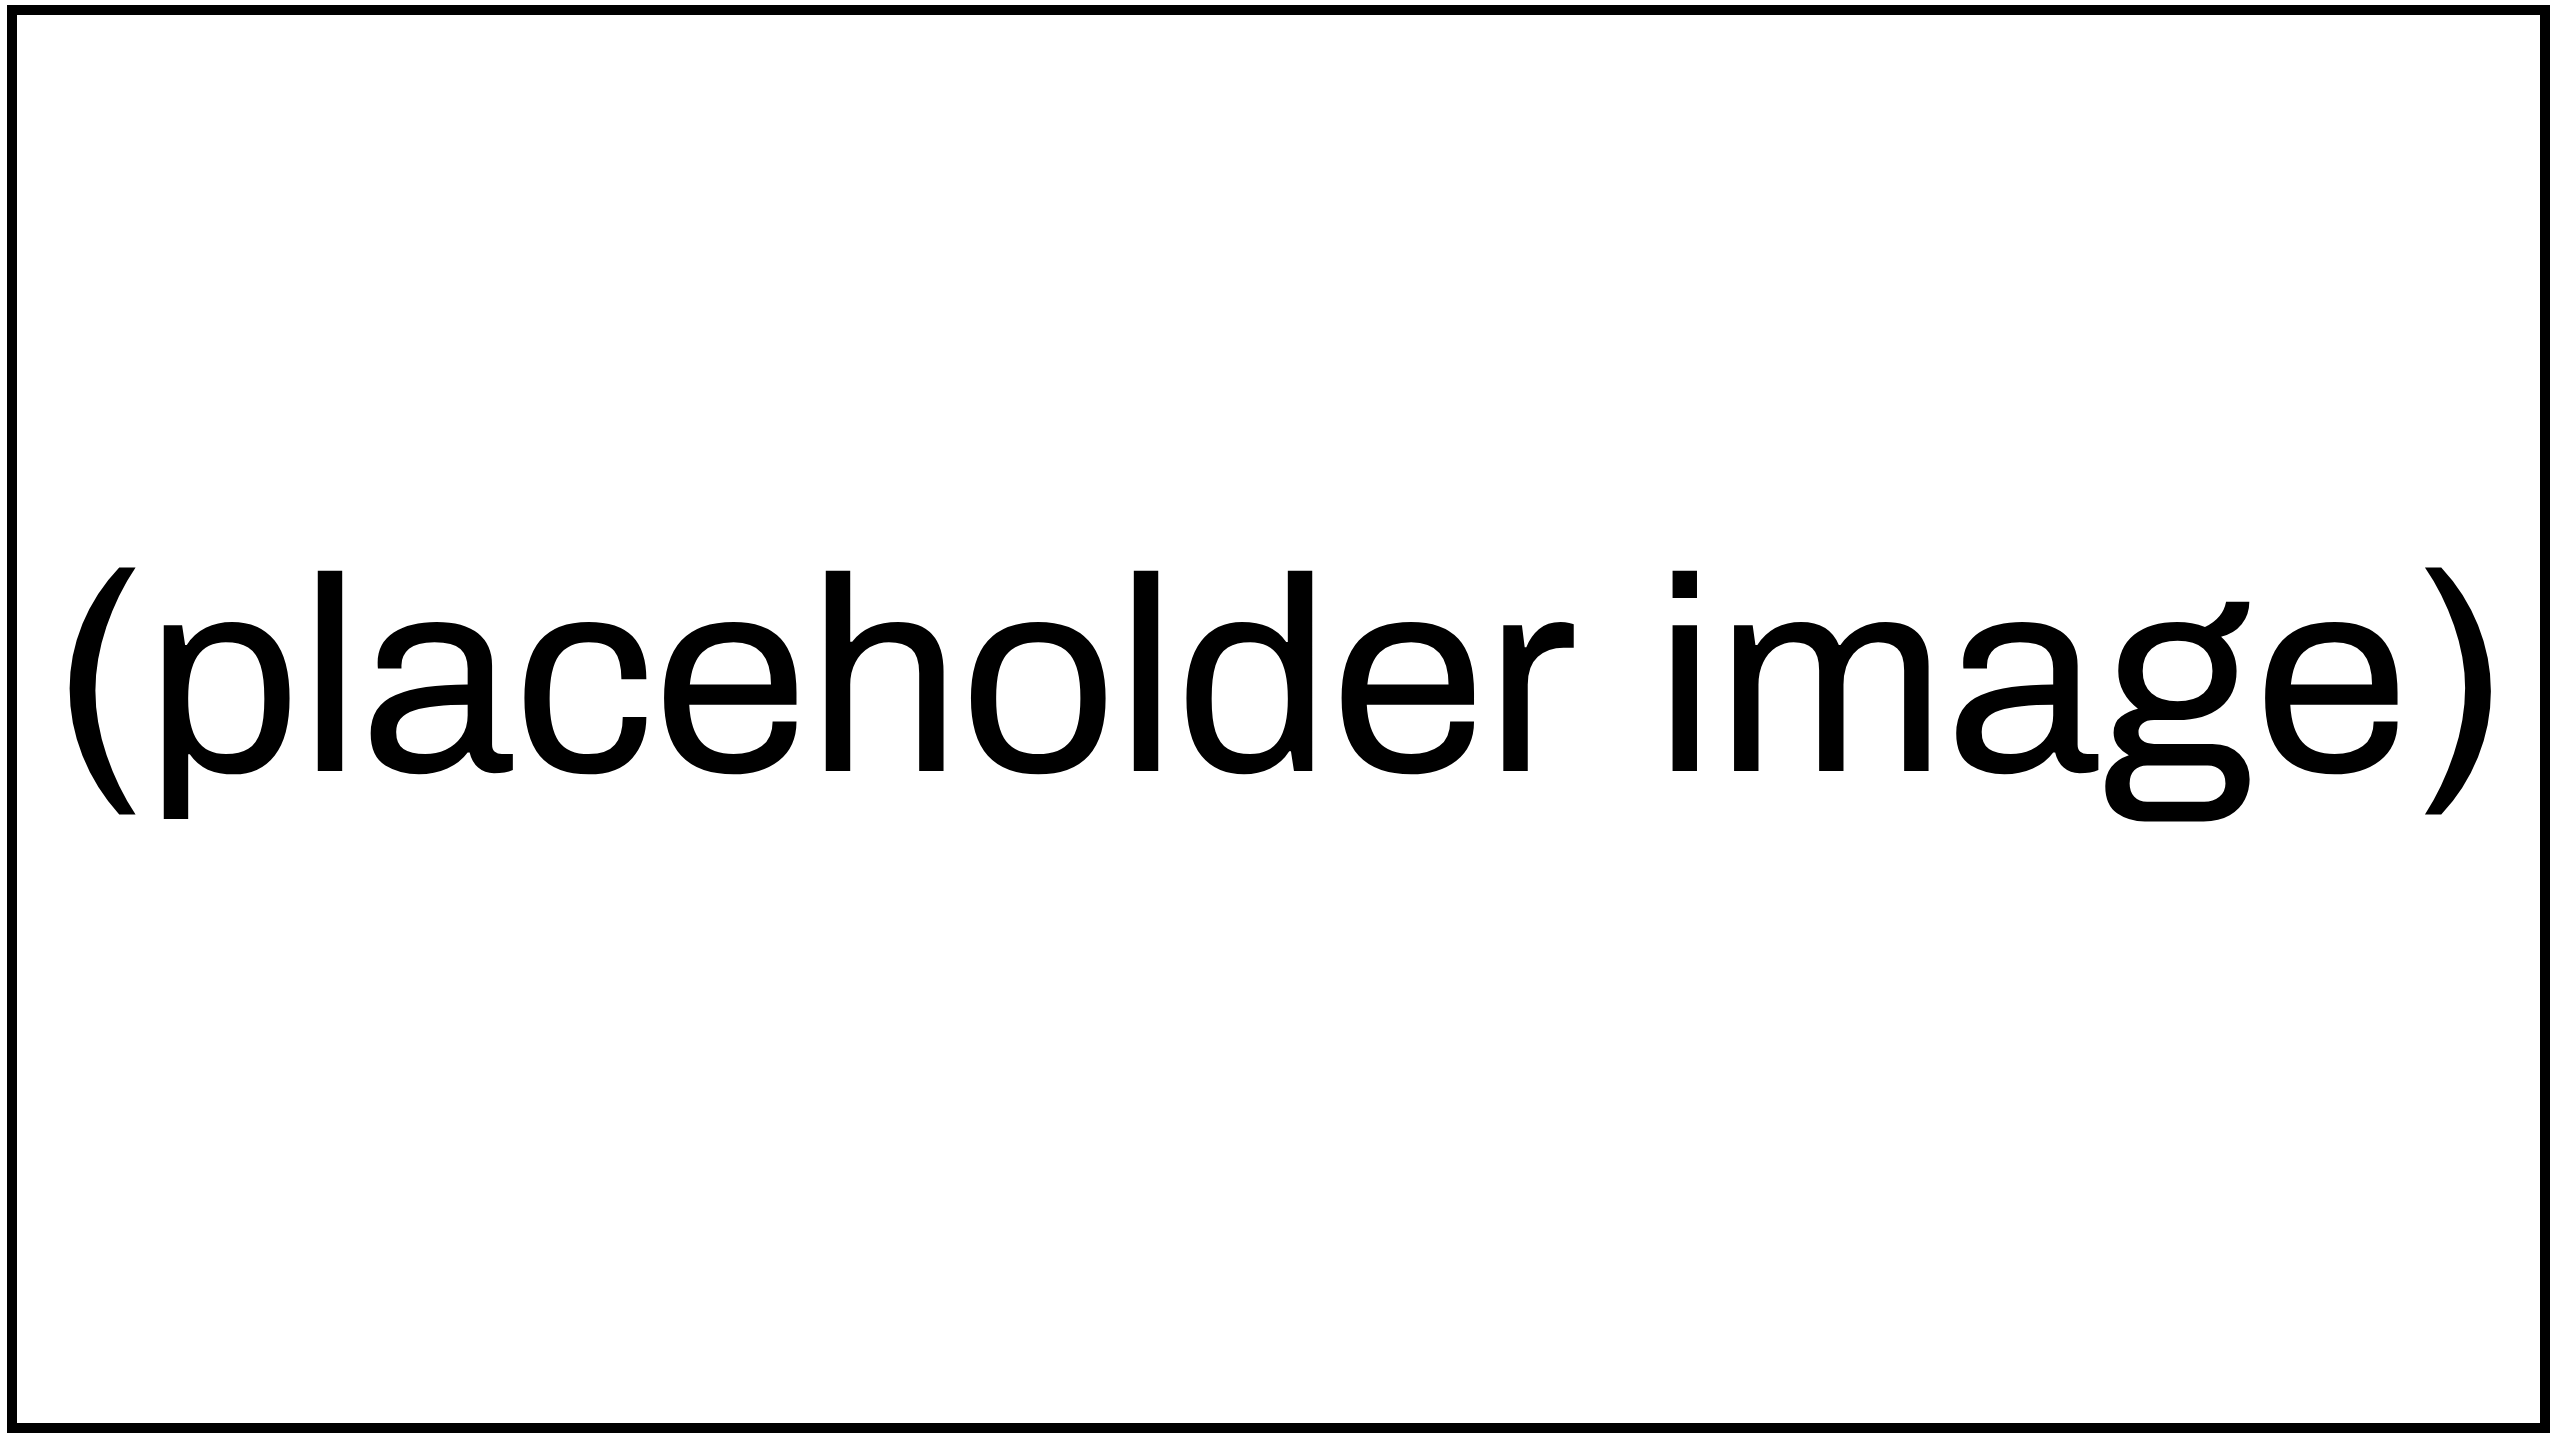
\includegraphics[width=0.8\textwidth]{figures/methodology/placeholder_image.png}
    \caption{SMKIT System Architecture Overview}
    \label{fig:system_architecture_overview}
\end{figure}

The diagram above illustrates how these components are structured and interact with one another to create a streamlined system for automating content generation and distribution.
\end{comment}

\subsection{Technological Stack}
\label{subsec:technological_stack}
The SMKIT project employs a variety of technologies and tools to ensure efficient and effective implementation of its components. The system's design relies primarily on \textit{Python}, a versatile programming language, which serves as the backbone for the development of all key modules. Below is a detailed description of the key technologies used in the project:

\begin{itemize}
    \item \textbf{Python}: \textit{Python} was selected as the primary programming language due to its ease of use, extensive library support, and suitability for web scraping, data manipulation, and automation tasks. The SMKIT system is built entirely in Python, utilizing its powerful libraries for a variety of tasks, from data extraction to content generation and posting.
    
    \item \textbf{argparse}: For managing command-line interfaces, the project uses the \textit{argparse} module. This module simplifies the process of handling command-line arguments, enabling users to interact with the system via terminal commands for various operations permitted by SMKIT.

    \item \textbf{BeautifulSoup}: \textit{BeautifulSoup} is used for web scraping tasks, specifically for extracting metadata and content from external websites. It simplifies the process of navigating HTML structures and retrieving relevant data from web pages.

    \item \textbf{matplotlib}: For visualizing data, the \textit{matplotlib} library is employed to generate plots and diagrams. This is particularly useful for representing the anger and conflict-based metrics derived from data.
    
    \item \textbf{facebook-sdk} and \textbf{tweepy}: These libraries are used to integrate the system with social media platforms like Facebook and Twitter, respectively. The \textit{facebook-sdk} allows for smooth interaction with the Facebook API for posting content, while \textit{tweepy} is used to manage content on Twitter. These libraries are integral in automating the process of sharing content on social media platforms, as discussed in Chapter 2.

\end{itemize}

Each of these technologies plays a vital role in the implementation of SMKIT, ensuring that the system operates efficiently, allowing for smooth data processing, content creation, and automation. The choice of Python, along with its extensive ecosystem of libraries, provides the flexibility needed to handle the diverse tasks within the system.

\subsection{Module Development for Negapedia Integration}
\label{subsec:module_development_for_negapedia_integration}
The integration of Negapedia data into the Social Media Kit (SMKIT) system is handled by a dedicated module, developed to enable the extraction, processing, and posting of content related to Negapedia articles. This integration follows a modular approach, allowing the system to load and interact with different data sources based on user input.

\begin{itemize}
    \item \textbf{Module Loading and Argument Management}: In SMKIT, the entry point is controlled via the command-line interface, using the \texttt{argparse} module to manage input parameters. A key parameter is \texttt{--module}, which specifies which data source module to load (e.g., \texttt{negapedia}). The system uses the \texttt{load\_module} function to dynamically load the appropriate module, ensuring flexibility and extensibility for future data sources.
    
    \item \textbf{Negapedia-Specific Input Validation}: When the \texttt{negapedia} module is selected, the system expects several mandatory input parameters, including \texttt{--pages}, \texttt{--post\_type}, \texttt{--mode}, and \texttt{--language}. These parameters are validated within the \texttt{handle\_module()} function of the Negapedia module. The function also includes checks specific to different posting modes, such as \texttt{summary}, \texttt{comparison}, and \texttt{ranking}, ensuring that the correct number of pages and ranking fields are provided before proceeding.

    \item \textbf{Data Extraction and Transformation}: Once the necessary parameters are validated, the Negapedia module extracts data from Negapedia pages, processing the content into a structured format, specifically a Python \texttt{TypedDict} called \texttt{NegapediaPageInfo}. This structure ensures that key information, such as words, conflict awards, polemic awards, and social jumps, is extracted and organized in a way that aligns with the system’s requirements. The amount of data to extract can be customized based on user input. The data transformation process then ensures that the raw Negapedia data, encapsulated in the \texttt{NegapediaPageInfo} dictionary, is usable for content creation and social media posting.
    
    \item \textbf{Post Settings and Customization}: The Negapedia module also allows customization of the posts to be generated. This includes setting the language, defining custom messages, and selecting the social media platforms (e.g., Twitter, Facebook) where the content will be posted. The settings are passed from the command-line arguments to the module, ensuring that each post aligns with user preferences.

    \item \textbf{Post Settings and Customization}: The Negapedia module also allows customization of the posts to be generated. This includes setting the language and eventually defining custom messages. For each language, a specific template is used, which is particularly tailored for the Negapedia module. These templates are designed to handle and display specific data, such as conflict awards, polemic awards, and social jumps, ensuring that the content is presented in a contextually relevant way for the target audience. The settings are passed from the command-line arguments to the module, ensuring that each post aligns with user preferences and the unique structure of the Negapedia content.
\end{itemize}

In summary, the integration of the Negapedia module within SMKIT is designed to be flexible, allowing the system to process and post content from Negapedia based on user-defined parameters. The module's dynamic loading system, combined with robust input validation and data transformation capabilities, ensures that the system can effectively generate relevant and customized social media content.

\section{Data Collection and Preparation}
\label{sec:data_collection_and_preparation}
This section describes how data is gathered, processed, and prepared for use in the SMKIT system. The process involves extracting raw data from web pages using web scraping tools, cleaning the data to ensure quality and relevance, and transforming it into a structured format that can be easily used for content generation and social media posting.

\subsection{Web Scraping Tools and Techniques}
\label{subsec:web_scraping_tools_and_techniques}
The primary web scraping tool used in SMKIT is \textbf{BeautifulSoup}, a Python library that facilitates the easy extraction of data from static HTML web pages. BeautifulSoup was chosen for its simplicity and effectiveness in handling static content, which is all that SMKIT requires, as the system does not need to handle JavaScript-rendered content.
The tool is used to parse the HTML content of web pages, extracting relevant data such as text, links, images, and metadata, and structuring it for further processing. BeautifulSoup works efficiently with both the generic module and the Negapedia module, as both modules rely on static HTML pages that can be parsed directly, without requiring complex JavaScript handling.
This approach is well-suited for the needs of SMKIT, as it allows for the extraction of critical data points like page titles, descriptions, and specific metrics for Negapedia (such as conflict or polemic awards), which are then processed into structured formats.

\subsection{Data Cleaning}
\label{subsec:data_cleaning}
After the raw data is collected from web scraping, it undergoes a cleaning process to ensure that it is accurate, relevant, and in a usable format for further processing. The cleaning process varies slightly between the generic module and the Negapedia module, based on the type of data being handled.

\begin{itemize}
    \item \textbf{Generic Module Cleaning}: In the case of the generic module, the data is parsed and structured using metadata tags such as \texttt{og:title}, \texttt{og:description}, \texttt{og:image}, etc., along with any fallback values (e.g., page title or URL) if these tags are missing. While no direct filtering is applied, the content is organized into a \texttt{PageInfo} structure for consistent processing and usage.
    
    \item \textbf{Negapedia Module Cleaning}: For the Negapedia module, data cleaning is more complex. A helper function, \texttt{filter\_data()}, is used to filter the data based on several criteria, such as the type of data (e.g., conflict or polemic), the category of the content (e.g., "all" or specific categories), and the period of the content. The filter ensures that only the most relevant data is selected for further processing, excluding irrelevant or outdated entries.
\end{itemize}

The data cleaning process ensures that only high-quality, relevant data is used in the system, avoiding the inclusion of outdated or irrelevant content.

\subsection{Data Transformation}
\label{subsec:data_transformation}
Once the raw data is cleaned, it is transformed into a structured format that can be easily used by SMKIT for content creation and social media posting. This process involves converting unstructured or semi-structured data into well-defined data types, which can be processed by the system’s components.

\begin{itemize}
    \item \textbf{Generic Module Transformation}: For the generic module, the cleaned data is converted into the \texttt{PageInfo} data type, which is a \texttt{TypedDict} in Python. The \texttt{PageInfo} structure includes fields such as \texttt{title}, \texttt{description}, \texttt{message}, \texttt{images}, \texttt{urls}, and \texttt{updated\_time}, among others. This structured format allows for easy access and manipulation of the data within the system.
    \item \textbf{Negapedia Module Transformation}: For the Negapedia module, the cleaned data is transformed into the \texttt{NegapediaPageInfo} data type, another \texttt{TypedDict} in Python. The \texttt{NegapediaPageInfo} structure is more complex, as it includes additional fields specific to Negapedia, such as \texttt{historical\_conflict}, \texttt{historical\_polemic} along with \texttt{social\_jumps} and \texttt{words\_that\_matter}, among others. These fields capture detailed metrics and visual representations of conflict, polemic, and social interactions, making the data more specific to the Negapedia context.
\end{itemize}

In summary, the data collection, cleaning, and transformation process in SMKIT is designed to ensure that the system operates with high-quality, structured data that is ready for use in content generation. By utilizing web scraping, applying filtering techniques for data cleaning, and transforming the data into structured formats like \texttt{PageInfo} and \texttt{NegapediaPageInfo}, SMKIT is able to automate the creation of social media content that is both relevant and contextually appropriate.


\section{Challenges and Limitations}
\label{sec:challenges_and_limitations}
This section discusses any technical, logistical, or methodological challenges encountered during the project, as well as the limitations of SMKIT.

\subsection{Technical Challenges}
\label{subsec:technical_challenges}
During the development of SMKIT, several technical challenges came up. These challenges were addressed with varying degrees of success, and some remain ongoing considerations for future improvements. One of the most significant technical difficulties encountered was related to integrating with social media APIs. The following points summarize the challenges related to social media API integration:

\textbf{Social Media API Integration:} Integrating with social media APIs such as Twitter and Facebook posed several difficulties. These difficulties derived from the complexities of working with third-party APIs and ensuring smooth interaction between SMKIT and the social media platforms. Key challenges included:

\begin{itemize}
    \item \textbf{Rate Limits:} Both Twitter and Facebook impose strict rate limits on API calls, restricting the number of requests that can be made within a given time frame. For example, Twitter limits the number of tweets that can be posted or retrieved within an hour, and Facebook places limits on the number of API requests for posting content or retrieving user data. These rate limits occasionally disrupted the real-time processing of data and timely posting of content, particularly on Twitter, where the restrictions are more stringent. It's important to note that while these rates are generally sufficient for typical usage of SMKIT, during development and testing, the rate limits on Twitter were occasionally reached.

    \item \textbf{Authentication Issues:} Handling OAuth authentication for accessing social media accounts was another challenge. Both Twitter and Facebook require OAuth 2.0 for user authentication, which involves obtaining access tokens that must be securely managed. Specifically, SMKIT had to deal with the complexities of managing long-lived tokens and refreshing expired tokens to maintain a continuous connection to the social media accounts. All possible authentication scenarios were covered by following the official documentation and implementing the necessary checks for token expiration, renewal, and error handling. In cases of token expiration or other authentication issues, SMKIT logs all relevant details, ensuring that the system can handle these situations appropriately. Although token expiration occasionally led to failures in posting or retrieving data, the system is designed to recover gracefully. Future improvements could include more robust token management systems.

    \item \textbf{Platform-Specific Restrictions and Features:} Each social media platform has its own unique set of features, restrictions, and guidelines for posting content. For example, Twitter limits the length of tweets and the number of images that can be attached, while Facebook has specific image and video size requirements for posts. SMKIT had to account for these platform-specific limitations when generating posts, ensuring that content was formatted correctly for each platform. This involved sometimes adapting data retrieval from the common structured format and other times working with platform-specific templates.

\end{itemize}

\subsection{Limitations of SMKIT}
\label{subsec:limitations_of_smkit}
Despite its capabilities, SMKIT has several limitations that need to be addressed in future versions of the tool. The following points outline the key limitations:

\begin{itemize}
    \item \textbf{Limited Social Media Platform Support:} Currently, SMKIT only supports posting on Facebook and Twitter. Other social media platforms such as Instagram, LinkedIn, or more specialized platforms are not yet supported.
    
    \item \textbf{Limited Metadata Extraction:} Although SMKIT extracts key Open Graph and HTML meta tags, it currently does not support a large range of metadata types or advanced features like full-page scraping (e.g., handling JavaScript-rendered content).
    
    \item \textbf{Lack of Real-Time Content Monitoring:} Currently, SMKIT does not provide real-time monitoring for changes on websites, such as Negapedia or any other website that uses Open Graph tags. Users must manually initiate the tool to check for new content or posts. Future versions could include automated monitoring and alerts.
\end{itemize}


\section{Conclusion}
\label{sec:methodology_conclusion}
This chapter provided a comprehensive overview of the methodology employed in the development of the Social Media Kit (SMKIT). The key points of the methodology are summarized below:

\begin{itemize}
    \item \textbf{System Design and Architecture:} The SMKIT system was designed with scalability and flexibility in mind. A modular architecture was adopted, allowing the tool to evolve with future requirements and support additional social media platforms or data sources.
    \item \textbf{Data Collection and Processing:} Data extraction was achieved using web scraping techniques, notably with BeautifulSoup for handling static HTML content. The data was then cleaned and transformed into structured formats suitable for content generation.
    \item \textbf{Implementation Process:} SMKIT’s implementation process involved integrating components like Negapedia and social media platforms through APIs. This ensured the automated creation and posting of content on platforms like Facebook and Twitter.
    \item \textbf{Challenges and Limitations:} The project encountered several challenges, particularly related to integrating with social media APIs, managing rate limits, and dealing with platform-specific restrictions. These challenges were mitigated through careful design and ongoing improvements.
\end{itemize}

Reflecting on the approach taken, the methodology ensured that the development of SMKIT was grounded in sound technical principles. The use of modular design provided flexibility, and the combination of web scraping and social media integration facilitated the core functionality of the tool.

Despite some limitations, including the lack of real-time monitoring and support for additional social media platforms, the methodology outlined in this chapter lays a strong foundation for future enhancements. The system is built to be extensible, and future improvements will address these limitations.

With a clear understanding of the tools, techniques, and challenges involved, the next chapters will delve deeper into the practical implementation of SMKIT, discussing the technical details of its construction.